\subsection*{a)}
	The circuit shown is a TTL (Transistor-Transistor Logic) implementation of a logical NOR gate. If either of the inputs is biased high, the input transistors will operate in reverse-active mode, and drive Q3 on, activating Q5 and hence pulling the output down. Only when both are low will Q4 be activated, pulling the output up.
\subsection*{b)}
	The totem-pole output stage provides low impedance driving to both high and low logical states, whilst also ensuring that the output will never be driven to both states simultaneously.
\subsection*{c)}
	The diode of the totem-pole output increases the turn on voltage present at the base of Q4, by raising the required emitter voltage by the diode $V_\mathrm{on}$. Hence, if transistor Q3 is on, which means the output should drive to low, or about 0 V, the voltage at the base of Q4 will be lowered by the resistance R2, typically to less than 1.4 V, and therefore turning Q4 off.
\subsection*{d)}
	$$ O = \lnot(A \lor B) $$
	\begin{figure}[htbp!]
		\centering
		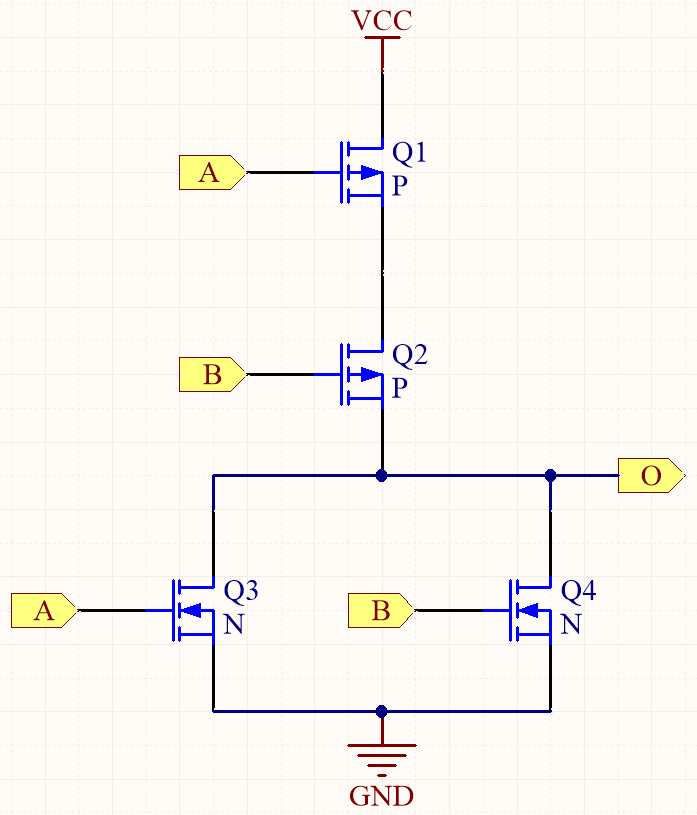
\includegraphics[height=0.4\textheight]{img/nor_gate}
		\caption{A CMOS implementation of a NOR gate.}
	\end{figure}